\begin{frame}{Process Context and \attack{} Classification}
    \small
    \raggedright
    \setlength{\parskip}{0pt}

    \begin{columns}[c,onlytextwidth]
        \column{0.39\linewidth}
        \begin{itemize}
            \setlength{\itemsep}{0.7em}
            \item Classify attack-related processes into \attack{} techniques.

            \item The same command can map to different techniques depending
                  on its execution context.

            \item Domain knowledge is encoded as explicit rules linking
                  context to technique labels.
        \end{itemize}

        \column{0.57\linewidth}
        \centering
        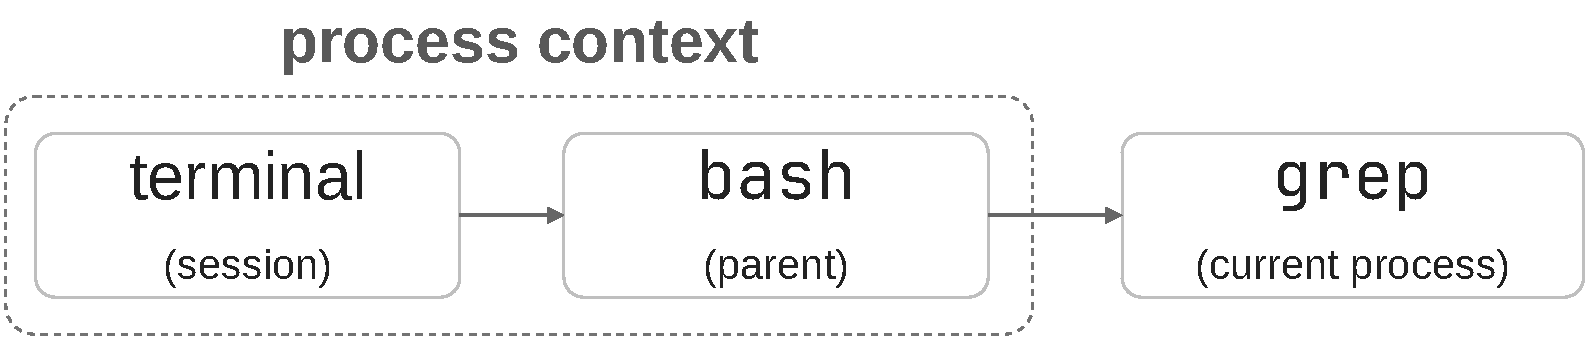
\includegraphics[width=0.98\linewidth]{figures/diagrams/process_context.pdf}
    \end{columns}
\end{frame}
